% !TEX TS-program = pdflatex
% !TEX encoding = UTF-8 Unicode

%************************************************
\chapter{Inquadramento storico}
\label{chp:Inquadramento storico}
%************************************************

\section{La nuova musica}
Nella storia della musica fino ai primi del novecento, si è diretto l’interesse verso una realtà compositiva legata all’universo tonale e ad un’armonia ferrea e rigorosa, così per la forma, fissa su nomenclature e ripartizioni classiche. Con il passare degli anni e con l’avvio della \textit{scuola di Darmstadt}, si sono andate ad ideare nuove tecniche compositive e ad inventare nuove forme stilistiche. Come scrive Henri Pousseur nelle conclusioni del suo libro \textit{Musica, semantica, società}:
\begin{quotation}
\textit{“ [...] quando è necessario, tagliare i rami che impediscono lo sviluppo armonioso dell’insieme, azione violenta in modo esemplare (purché prudente)! \\ 
L’arte moderna potrà sviluppare fin d’ora i modelli di ciò che Marcuse chiamerebbe il “lavoro libidinoso” (anticipando in tal modo esigenze di un stato di pace ancora sconosciuto), soltanto se non trascura di denunciare nello stesso tempo, nella maniera più efficace possibile, ciò che ancora impedisce (con la feroce durezza che sappiamo) a questo stato di pace e a questa possibilità di gioiosa creazione collettiva di diffondersi su tutta la faccia della terra! In questa prospettiva penso che è perfettamente lecito dar ancora prova di un po’ d’impazienza, di invitare con urgenza agli indispensabili scossoni. Anzi, sarebbe imperdonabile restare senza far nulla! Lo si voglia o no, il tempo dei flauti e delle cornamuse, di cui occorre intuire e far intuire la felicità, è attualmente ancora imperdito da quello della tromba, del tamburo e del Grido.” \footnote{Henri Pousseur, \textit{Musica, semantica, società}, traduzione di Eugenio Costa per Casa editrice Valentino Bompiani \& C. S.p.a., Milano, 1972}}
\end{quotation}
Di questa citazione bisogna selezionare alcune parti fondamentali, ed eventualmente puntare la nostra lente d'ingrandimento su delle questioni assai più complesse. L'idea di stralcio, di taglio, può avvenire solo nel caso non si fanno i conti con la tradizione e si renda del tutto inutile il legame con il passato. Questo, però, non avviene, dato che, per quanto il serialismo sia una tecnica che rompe con la tradizione, rimane legato a molte forme e a molti universi compositivi interni alla cultura classica: si cambiano le metodologie "armoniche", ma si rimane ferrei all'interno di schemi ben definiti. \\
\MakeUppercase{è} con la nascita di una figura importantissima per la musica contemporanea che si inizia a delineare un nuovo scenario legato al\textit{la nuova musica}: il \textbf{tecnico audio}. Lo studio di fonologia di Milano, lo studio di GRM di Parigi, Lo studio elettronico di Mosca, nella figura dell'ingegnere Eugenij Murzin, la nascita di molte radio legate agli studi di ricerca sul suono, sono i baluardi di questo immaginario sonoro nel quale oltre la musica scritta a livello notazionale si iniziano a scrivere algoritmi e schemi legati ai sistemi di diffusione. Il suono non è più delimitato all'interno di altezze legate al mondo temperato. Già con Ligeti, Hàba e Wyschnegradsky si concentrarono in Europa numerose esperienze teoriche, sperimentali e compositive che prevedevano l’uso di \textit{microintervalli}, grazie anche all'utilizzo del calcolatore, che rendeva possibile accostamenti ritmico-melodici difficili da concepire a livello classico (ad esempio l'accostamento di un vasto numero di oscillatori che differivano di pochi herz l'uno dall'altro o la nascita della modulazione di frequenza).\\
Lo stesso Bruno Maderna sostenne, durante un concerto presso Darmastadt del 1959, in riferimento ad una sua composizione, \textit{Musica su due dimensioni} (1952):

\begin{quotation}
[...] ho imparato che la musica è un'arte del tempo, perché fino al momento dell'esecuzione si deve dar forma e ordinare l'imprevedibile e perché io come compositore mi trovavo di fronte a me stesso come interprete. Nell'ambito della musica strumentale queste due funzioni sono state sempre più separate: io scrivo una partitura e la dò all'interprete, [...] la responsabilità della realizzazione sonora è nelle mani di un'altra persona dotata di proprie idee, e capacità. Una sintesi di entrambe le possibilità esistenti che io chiamo "dimensioni" mi sembra particolarmente fruttuosa, dal momento che l'interprete, nell'incontro con le realizzazioni sonore fissate sul nastro, fatte dallo stesso compositore o da lui controllate, raggiunge un contatto molto pi
 stretto con l'autore. [...] Io ho avvertito per la prima volta nel 1952 la necessità di questa sintesi, e ne fui felice, poiché ho sempre desiderato di collegare la composizione e l'interpretazione\footnote{Francesco Galante Nicola Sani, \textit{Musica Espansa, Percorsi elettroacustici di fine millennio}, Casa Ricordi LIM Ediitrice, 2000}.
\end{quotation}

Per Luigi Nono "la musica deve saper intervenire nella situazione contemporanea, nella storia contemporanea"\footnote{\textit{ibidem}} e così accade, anche grazie alla nascita di \textit{regie del suono} e figure come Alvise Vidolin, Antonio Farina, Nicola Bernardini e molti altri, prendono forma e rendono possibile pensare ad una composizione, oltre che nella sua natura di scrittura, anche come messa in scena. Così con il tempo si innesca un nuovo approccio alla musica e al suono che prese il nome di \textit{musica elettroacustica}.

\begin{quotation}
Nello studio elettronico si possono trovare direttamente diverse possibilità di concretizzazione di strutture sonore, che attraverso manipolazioni di concretizzazione di strutture sonore, che attraverso manipolazioni continue si possono rinnovare e mutare all'infinito [...], e come il tempo ora si presenti come un campo vastissimo di possibilità. Noi ora proviamo propensione a questo tipo di pensiero, non più lineare e di condotta presente anche nella musica strumentale [...]\footnote{\textit{ibidem}.}
\end{quotation}

Può apparire anche quasi antico il discorso che continuo a sottolineare in questo capitolo, dato che sembrano ormai ben saldi questi paradigmi e quasi alla base della musica elettroacustica che ogni giorno andiamo ad analizzare. Rimane però questo piccolo particolare, l'emozione per una cura al dettaglio, una cura alla necessità di esprimere un concetto, tramite un metodo. Sottolineo questo concetto, perché è proprio la cura al particolare, ma anche ad una calma interna, che dà la possibilità di soffermarsi su caratteri musicali e compositivi per me estremamente necessari come il timbro e le micro-variazioni tonali.

%************************************************************************************

\section{Il legame con il passato}

\subsection{Spettralismo}
Ad oggi, la business music ha rivelato migliaia di generi musicali legati alla musica elettroacustica ed elettronica ed è riuscita a catalogare in moltissimi insiemi e sottoinsiemi il mondo musicale. In passato, però, più che di genere musicale, si parlava di corrente artistica, prima che le etichette discografiche diventassero delle vere e proprie \textit{direzioni artistiche} e prima che si imponessero le leggi di mercato, si parlava appunto di correnti e in questo capitolo mi vorrei soffermare su una di esse: lo  \textit{spettralismo}. \\
Se con la nascita dello \textit{spettralismo} abbiamo la crescita di una musica composta per strumento ma resa più ricca timbricamente anche grazie all’ausilio dei computer, grazie all’analisi spettrale e alla possibilità di creare maglie di suoni fino a quel momento sconosciute, in seguito con la musica elettroacustica si ha la possibilità di unire questi due mondi creando un’ambiguità sonora notevole. \\
Nella maggior parte dei casi si andava a ricercare la modifica a livello di altezze e in qualche modo anche di "amplificare" le capacità timbriche di uno strumento tramite l’utilizzo di campionamenti differenti dei file di ripresa eseguiti in precedenza o tramite vari filtraggi, ricordiamo il brano per sassofono e nastro magnetico di Jean-Claude Risset: \textit{Voilements}. \\
Lo sviluppo di nuove tecnologie e di tempi di elaborazione del suono sempre più puntuali, ha reso possibile l'elaborazione del suono dal vivo e la possibilità di rendere sempre più complesse le creazioni degli \textit{algoritmi} presenti anche in partitura che venivano ideati dai compositori, come Luigi Nono, Luciano Berio, Michelangelo Lupone e moltri altri maestri della musica contemporanea che hanno utilizzato, nel connubio tra tecnica e arte, queste \textit{invenzioni compositive e tecnologiche}. \\
Proprio sulla base dello studio compositivo e tecnologico che mi vorrei soffermare. Ovviamente se uno strumento musicale viene utilizzato solo nelle sue tecniche classiche, il divario tra elettronica e strumento classico sarà difficile da colmare. Quindi, già nell’utilizzo della \textit{spazializzazione} che nell’elaborazione dal vivo, questo divario è diventato sempre più piccolo. Luciano Berio con i suoi studi sugli strumenti e in seguito Giorgio Netti e molti altri, tramite la scrittura e l’utilizzo di tecniche estese sempre più precise e complesse, sono arrivati al vivo dell’argomento. La risposta finalmente non è fuori, nell’utilizzo di un’elettronica troppo più potente degli strumenti canonici, ma è dentro, nella ricerca di tecniche estese che possano portare lo strumento ad essere vissuto in tutta la sua pienezza timbrica, frequenziale e di ampiezza sonora. 

\subsection{La ripresa microfonica}

Lo studio delle tecniche estese e la possibilità di cogliere qualunque sfumatura di uno strumento viaggia a pari passo con l’evoluzione della tecnologia. Finalmente microfoni creati \textit{ad hoc} per riprendere determinate qualità di uno strumento e una miriade di effetti di ambiente\footnote{riverberi a convoluzione, ad esempio}, diventano quasi un prolungamento dello strumento di liuteria classica. Questo non per sminuire l’interesse verso uno strumento musicale del quale possiamo apprezzare anche acusticamente le sue qualità, ma molto più per accentuare le qualità timbriche: una \textit{lente di ingrandimento sul suono}. C'è un importanza della ripresa microfonica anche a livello compositivo: il microfono in una nuova modalità deve diventare fido compagno del compositore, il quale, dovrebbe iniziare ad apprezzare ogni strumento non solo nella sua natura acustica ma anche nel suo \textit{essere amplificato}. In un’idea ormai antica ma mai rimarcata: \\
\[\textbf{strumento musicale + microfonazione}\] \\
Fausto Romitelli, compositore rimasto in attività fino al 2004, esigeva la microfonazione dei suoni strumentisti e non disdegnava l'utilizzo di uno svariato numero di diffusori. In \textit{Professor Bad Trip, Lesson I} possiamo vedere come una soluzione ritmico-melodica è scritta per far assaporare un fittizio \textit{eco} da parte degli archi tramite una ripetizione e una diminuzione graduale del volume indotto negli attacchi: 
\begin{figure}[htbp]

\begin{center}

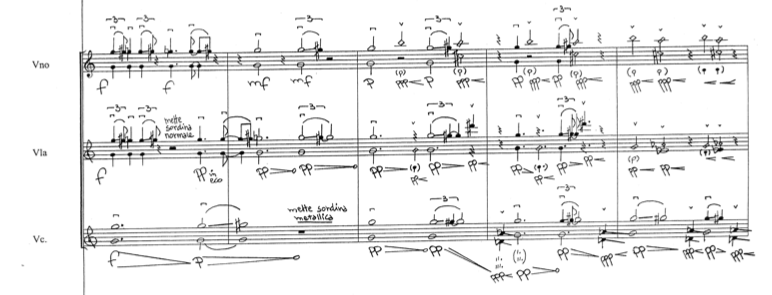
\includegraphics[width=1.\textwidth]{Romitelli_01.png}

\caption{particolare partitura \textit{Professor Bad Trip, Lesson I}}

\label{fig:01_Romitelli}

\end{center}

\end{figure}

La presenza del microfono diventa, come detto, una vera e propria lente di ingrandimento sul suono, che ci fa apprezzare e trasformare in arte compositiva e quindi in gesto, anche le micro-variazioni frequenziali e di ampiezza e di spettro che lo strumentista va ad eseguire. Ciò ha portato a partiture più accurate e con questo ad una maggiore attenzione da parte dello strumentista a cogliere fino alle più piccole sfumature legate allo strumento.

\begin{quotation}
Una netta contrapposizione - in suoni di combinazione - tra stabilità (suono normale) e instabilità (suono raschiato) porta a inaspettate e sorprendenti relazioni certamente da considerare - tra le altre - come primarie\footnote{Simone Santi Gubini, \textit{Difettosità timbrica e subarmoniche}, Masterclass Emufest  2017, Roma}.
\end{quotation}

\subsection{L'elettronica}

La parte riservata all’elettronica in questo caso diviene un ulteriore supporto, se non proprio un ulteriore indagine verso nuove idee compositive. Non c’è più bisogno di ricercare negli intervalli armonici o inamornici dei cavilli per uscire o rientrare in un panorama moderno, si può lavorare in micro-mondi atonali che si muovono anche all’interno di una o due note\footnote{N.B.: in questo caso parlo di nota non per indicare l'universo temperato, ma solo per semplicità: lavorare su altezze molto vicine, che poi siano note precise come un do, o che sia un do monesis calante o un fa, poco importa. Il fine è il raggiungimento di una nostra soluzione compositiva, con la quale, partitura dopo partitura, riusciamo a redigere un corollario di gesti e notazioni che, se spiegate, si possono eseguire di nuovo alla stessa maniera. \\}. Ovviamente, i grandi maestri come Nono ci indicano il cammino e rendono possibile avere una traiettoria, una base, dalla quale poter partire:

\begin{quotation}
Per esempio si prenda un suono, Si\textit{b.} Oggi è possibile con la tecnologia, con il \textit{live electronics} (o senza) utilizzare una parte del suono, una parte dell'aria o, improvvisamente, tutto il suono, con una direzione particolare e un'intensità particolare, fino a terminare solamente con un soffio. Allora non c'è più un Sib, ma il flautista viene a utilizzare il soffio più vicino al Si\textit{b}, e il \textit{live electronics} permette di esaltarlo. Tutto questo è ciò che con la tecnica si può ottenere oggi da un solo suono che eravamo abituati a considerare molto preciso, uniforme, unitario. [...]  è impossibile riconoscere il cambiamento di un clarinetto contrabbasso a una tuba a sei pistoni, o a un mezzosoprano, quando suonano estremamente piano. Non è possibile per il motivo che tutti gli strumenti, tutte le sovrapposizioni degli elementi armonici del suono, scompaiono\footnote{Luigi Nono, \textit{La nostalgia del futuro, Scritti scelti 1948-1986}, Gruppo editoriale Il Saggiatore s.p.a., Milano 2007}.
\end{quotation}

La notazione rediviva si colora di metodo, sempre più incalzante, sempre più denso di nozioni che servono a far intendere ciò che il compositore vuole e dove vuole arrivare, la piena coscienza del suono e delle modalità di esecuzione per arrivare a tali corrispondenze. \\
\textit{Insinuarsi nel vuoto} è il nome con il quale ho marchiato questo \textit{dittico}, un viaggio in due mondi, paralleli e lontani, ma limitrofi e adiacenti, nei quali provo ad unire suoni lontani, quasi atavici, in complesse (almeno per me) forme musicali. Nei capitoli successivi andrò a sviscerare la comparazione tra strumenti classici e \textit{Unamolla}, così da rendere più coscienzioso e intimo il contatto con la parte compositiva, perché solo penetrando e passando al microscopio alcune parti della materia, si può cogliere a pieno il suono che, tramite la diffusione, si disperde nell'aria. Concludo con una citazione da \textit{On Sonic Art} di Trevor Whishart, che si riferisce a questo campo e riguarda uno strumento ancestrale, quanto contemporaneo: la voce.

\begin{quotation}
[...] musical gesture is evidenced in the internal morphology of sound-objects and also in the overall shaping of groups, phrases, etc. [...] the morphology of intellectual-physiological gestures [...] may be translated directly into the morphology of sound objects by the action of the larynx, or the musuclature and an instrumental transducer. The translation of performance-gesture into the gestural-structure of the sound-object is most complete and convincing where the technology of instrument construction does not present a barrier\footnote{Trevor Wishart, \textit{On Sonic Art, a new and revised edition edited by Simon Emmerson}, Published in The Netherlands by Harwood Academic Publishers, Amsterdam, 1996}.
\end{quotation}





